\section{Unified Multi-Mode Architecture \& Top-Level Controller}
\label{sec:architecture}

The deployment of the Module-Lattice-Based Key-Encapsulation Mechanism (\mbox{ML-KEM}) across resource-constrained cyber-physical edge devices, high-assurance Hardware Security Modules (HSMs), and high-throughput datacenter security enclaves necessitates a radical departure from conventional domain-specific coprocessor architectures. In traditional post-quantum cryptographic (PQC) hardware designs, dedicated, siloed execution datapaths are frequently instantiated for each cryptographic primitive: Key Generation (\mbox{KeyGen}), Encapsulation (\mbox{Encaps}), and Decapsulation (\mbox{Decaps})~\cite{xing2023tcas1, imran2022tvlsi}. Although conceptually straightforward and modular, this decoupled methodology incurs prohibitive silicon area overheads, replicates complex arithmetic functional units, and rapidly depletes embedded Block RAMs (BRAMs).

To overcome these fundamental microarchitectural bottlenecks, this work introduces a fully unified, monolithic controller and datapath core encapsulated within the top-level module \texttt{mlkem\_keygen\_top}. The proposed architecture executes all three standardized \mbox{ML-KEM} operations specified in NIST FIPS~203~\cite{fips203}---Key Generation (Algorithm~16/19), Encapsulation (Algorithm~17/20), and Decapsulation with Implicit Rejection (Algorithm~18/21)---across all three security categories (\mbox{ML-KEM-512}, \mbox{ML-KEM-768}, and \mbox{ML-KEM-1024}) within a single consolidated hardware datapath. By aggressively multiplexing a four-butterfly parallel Number Theoretic Transform ($\text{NTT}$) engine, an eight-DSP dual-channel Karatsuba pointwise multiplier, a 24-cycle $\text{Keccak-}f[1600]$ cryptographic sponge, and unified polynomial serialization codecs, the presented design accomplishes complete algorithmic acceleration under an ultra-constrained hardware budget of \textbf{strictly zero Block RAMs ($0\text{ BRAM}$)} and \textbf{strictly eight DSP slices ($8\text{ DSP48E2}$)}, while sustaining an operating clock frequency of $413.7\text{ MHz}$ on an AMD Kintex UltraScale FPGA.

\subsection{System Microarchitecture \& Monolithic Design Philosophy}
\label{sec:arch_microarchitecture}

The top-level microarchitecture of the proposed accelerator is depicted in Fig.~\ref{fig:top_controller}. The core is encapsulated within the monolithic module \texttt{mlkem\_keygen\_top}, which integrates the subordinate encapsulation datapath (\texttt{mlkem\_encap\_datapath.svh}) and decapsulation datapath (\texttt{mlkem\_decap\_datapath.svh}). The hardware interfaces with the host computing platform via an asynchronous-reset, synchronous-clock streaming architecture engineered for high-bandwidth, deterministic cryptographic execution.

\begin{figure*}[!t]
\centering
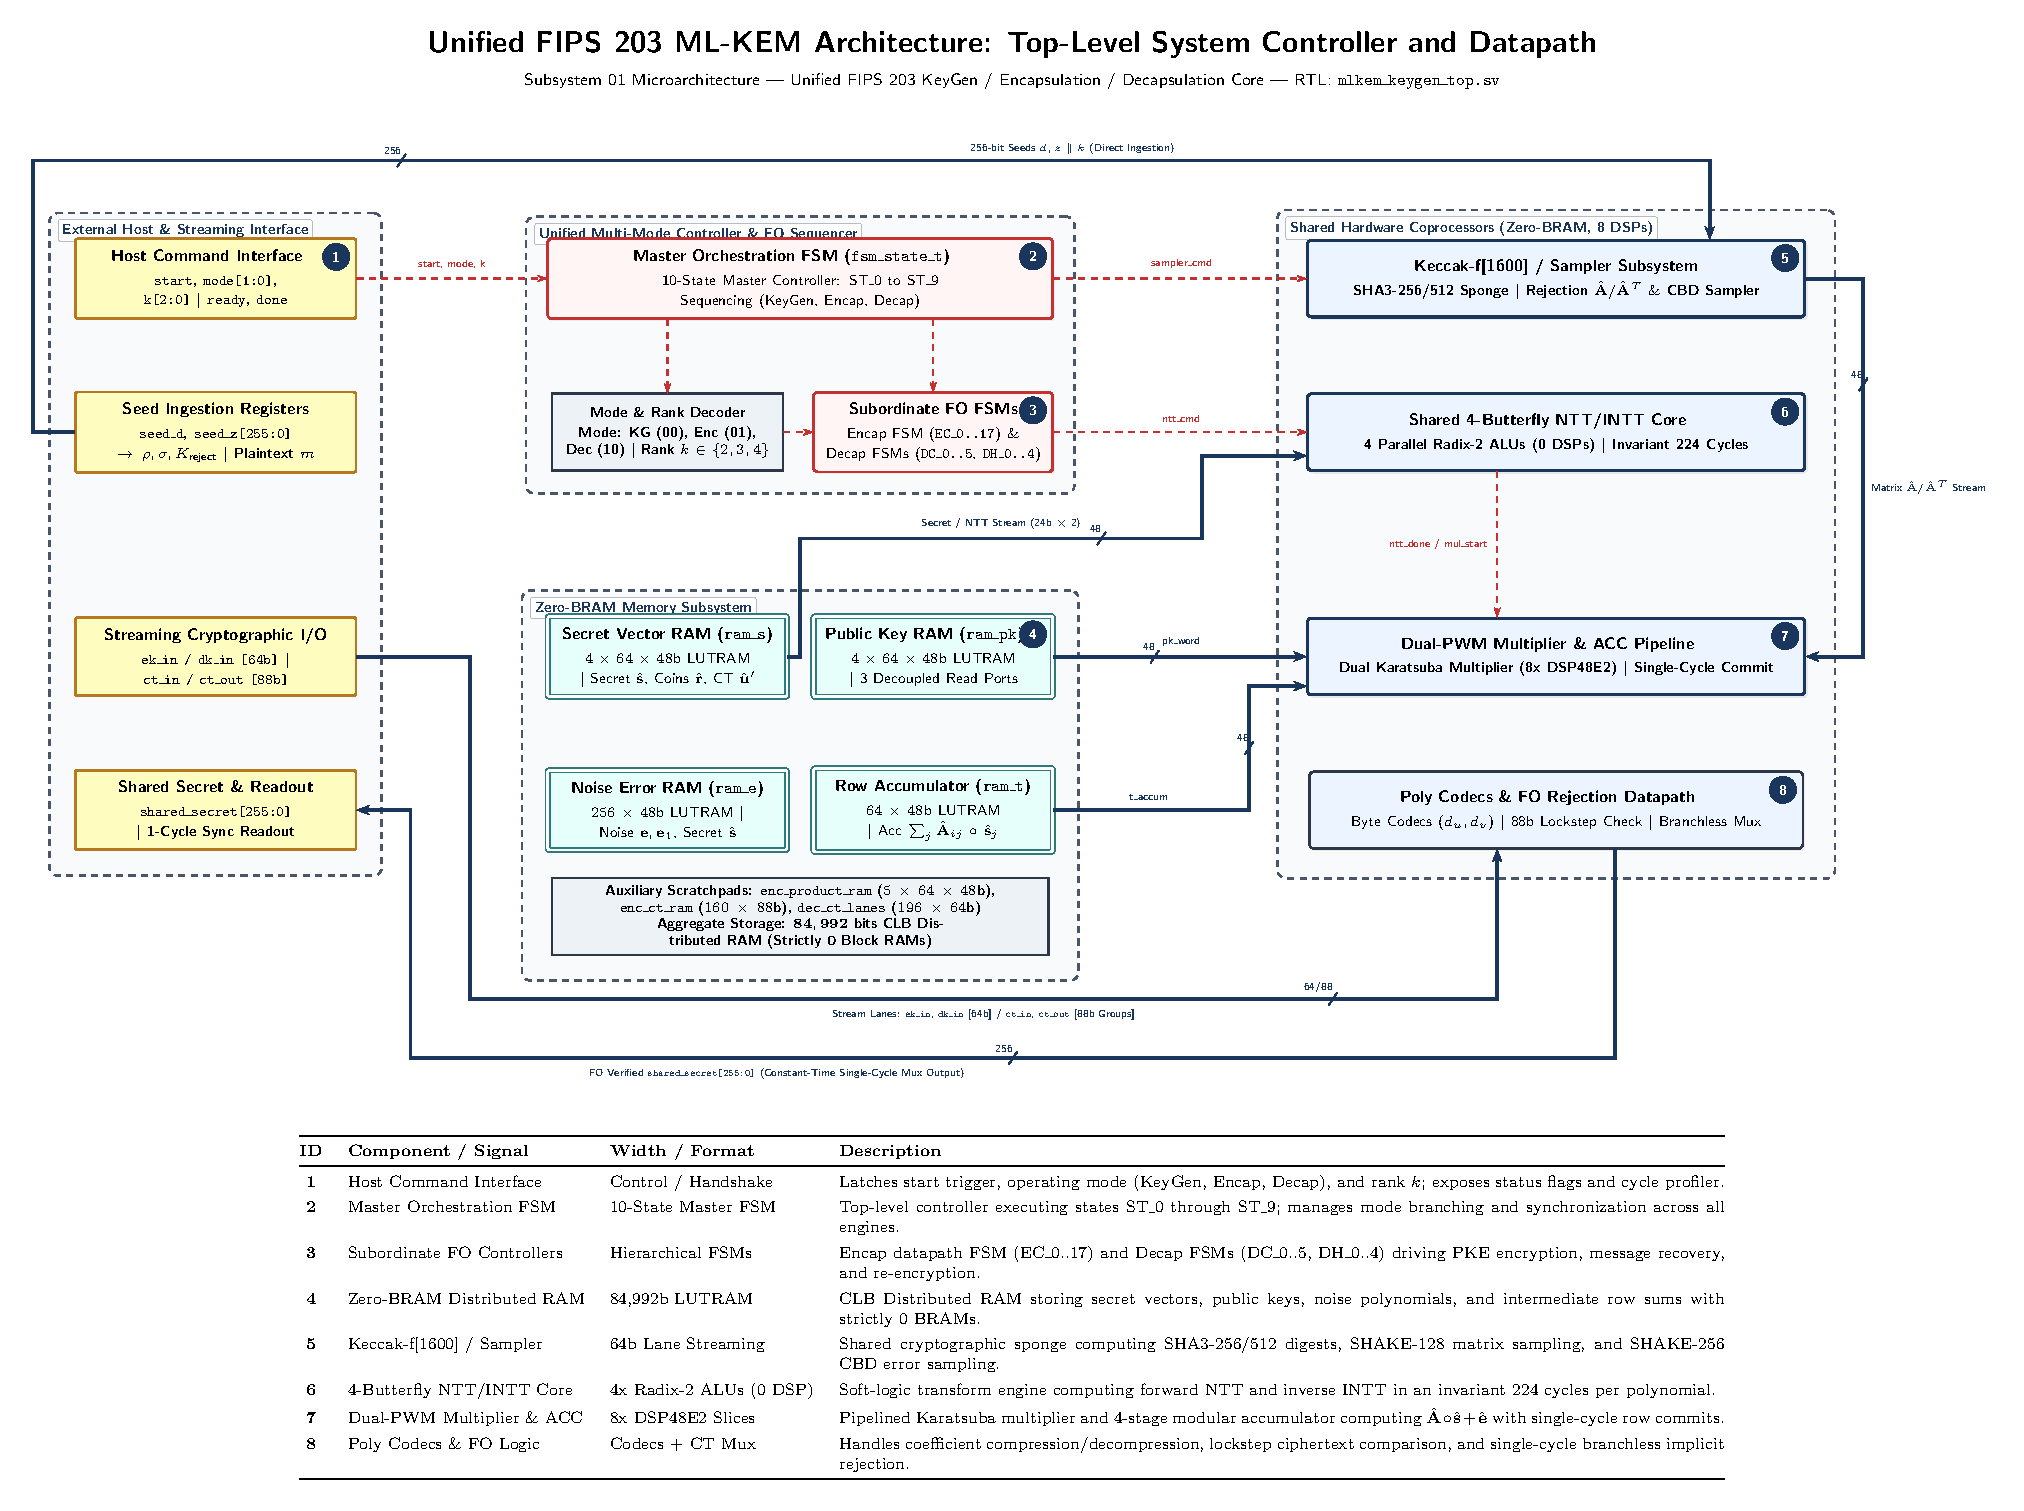
\includegraphics[width=\textwidth]{figures/fig01_top_controller.pdf}
\caption{Unified top-level system architecture and multi-mode controller for NIST FIPS 203 (\mbox{ML-KEM}), partitioned into three primary architectural columns: 1)~External Host \& Streaming Interface (Left), providing synchronous command handshaking, 256-bit seed ingestion, 64-bit streaming key channels, 88-bit ciphertext buses, and 1-cycle RAM readout; 2)~Unified Multi-Mode Controller \& Zero-BRAM Memory Subsystem (Center), orchestrating execution through the 10-state master FSM (\texttt{fsm\_state\_t}), mode/rank decoders, subordinate FO sequencers, and an $84,992\text{-bit}$ distributed LUTRAM memory hierarchy; and 3)~Shared Hardware Coprocessors (Right), integrating the 24-cycle Keccak-$f[1600]$ sponge, 4-butterfly parallel NTT/INTT transform engine, 8-DSP dual-channel Karatsuba multiplier, and constant-time Fujisaki-Okamoto (FO) verification datapath.}
\label{fig:top_controller}
\end{figure*}

The microarchitectural partition comprises three functional columns:
\begin{enumerate}
    \item \textbf{External Host \& Streaming I/O Subsystem (Column 1):} Manages command/configuration ingestion, entropy seeding ($d, z$), streaming encapsulation/decapsulation keys ($ek, dk$), compressed ciphertext transfers ($ct$), and deterministic memory readout.
    \item \textbf{Unified Multi-Mode Controller \& Zero-BRAM Memory Subsystem (Column 2):} Houses the master 10-state orchestration finite state machine, rank decoders, subordinate FO transform sequencers, and $84,992\text{ bits}$ of distributed LUTRAM arrays.
    \item \textbf{Shared Computational Coprocessors (Column 3):} Encompasses the cryptographic sponge and rejection sampler, the parallel transform ALU, the streaming pointwise multiplier with its 4-stage modular accumulator, and the constant-time implicit rejection comparator.
\end{enumerate}

By consolidating control and datapath logic into a single monolithic entity, our design completely avoids the interconnect routing congestion, inter-module latency penalties, and peripheral interface duplication typical of multi-core PQC implementations.

\subsection{Physical Pinout \& Handshake Protocols}
\label{sec:arch_pinout}

The physical pinout and interface protocol of \texttt{mlkem\_keygen\_top} are structured to decouple control sequencing from wide cryptographic data streams. Table~\ref{tab:pinout} details the complete physical interface specifications, signal directions, word widths, clock domains, and protocol handshaking behaviors.

\begin{table*}[!t]
\caption{Complete Physical Interface Pinout and Signal Handshake Specification for \texttt{mlkem\_keygen\_top}}
\label{tab:pinout}
\centering
\footnotesize
\begin{tabular}{@{} l c c l p{8.2cm} @{}}
\toprule
\textbf{Port Identifier} & \textbf{Dir} & \textbf{Width (b)} & \textbf{Clock Domain} & \textbf{Description \& Handshake Protocol} \\
\midrule
\multicolumn{5}{@{}l}{\textit{\textbf{1. Global Control, Mode Configuration, and Status Interface}}} \\
\addlinespace[2pt]
\texttt{clk} & In & 1 & System Clock & Nominal 450.0~MHz, achieved post-route 413.7~MHz on Kintex UltraScale. \\
\texttt{rst\_n} & In & 1 & Asynchronous & Active-low global asynchronous hardware reset. \\
\texttt{start} & In & 1 & \texttt{clk} (rising) & Single-cycle execution initiation pulse; sampled when \texttt{ready} is asserted high. \\
\texttt{ready} & Out & 1 & \texttt{clk} (reg) & Core idle indicator; asserts high when controller can accept new operation commands. \\
\texttt{done} & Out & 1 & \texttt{clk} (reg) & Operation completion flag; asserts high upon valid execution termination. \\
\texttt{mode[1:0]} & In & 2 & \texttt{clk} (latched) & Operational primitive selector: \texttt{2'b00} (KeyGen), \texttt{2'b01} (Encap), \texttt{2'b10} (Decap). \\
\texttt{k[2:0]} & In & 3 & \texttt{clk} (latched) & Module rank selector: \texttt{3'd2} (ML-KEM-512), \texttt{3'd3} (ML-KEM-768), \texttt{3'd4} (ML-KEM-1024). \\
\texttt{seed\_d[255:0]} & In & 256 & \texttt{clk} (latched) & 32-byte uniform random seed $d$ ingested during KeyGen for ($\rho, \sigma$) expansion. \\
\texttt{seed\_z[255:0]} & In & 256 & \texttt{clk} (latched) & 32-byte seed $z$ ingested for rejection key derivation ($K_{\text{reject}}$) and private key serialization. \\
\texttt{enc\_message[255:0]} & In & 256 & \texttt{clk} (latched) & 32-byte plaintext message $m$ supplied to encapsulation datapath for shared key derivation. \\
\texttt{operation\_error} & Out & 1 & \texttt{clk} (reg) & Error flag; pulses high upon detecting noncanonical coefficients ($\ge 3329$) or rank framing faults. \\
\texttt{shared\_secret[255:0]} & Out & 256 & \texttt{clk} (reg) & 256-bit symmetric session key (valid $K$ or pseudorandom $K_{\text{reject}}$ via branchless multiplexer). \\
\texttt{cycle\_cnt[31:0]} & Out & 32 & \texttt{clk} (reg) & Real-time performance counter; records exact active clock cycles from \texttt{start} to \texttt{done}. \\
\midrule
\multicolumn{5}{@{}l}{\textit{\textbf{2. High-Bandwidth Streaming Key and Ciphertext Ingestion/Emission Lanes}}} \\
\addlinespace[2pt]
\texttt{ek\_in\_valid} & In & 1 & \texttt{clk} & Streaming public key valid handshake strobe. \\
\texttt{ek\_in\_ready} & Out & 1 & \texttt{clk} & Backpressure credit; indicates accelerator readiness to ingest public key lane. \\
\texttt{ek\_in\_data[63:0]} & In & 64 & \texttt{clk} & 64-bit little-endian public key slice ($48k + 4$ total lanes ingested). \\
\texttt{ek\_in\_last} & In & 1 & \texttt{clk} & Packet boundary delimiter; marks final public key slice transfer. \\
\texttt{dk\_in\_valid} & In & 1 & \texttt{clk} & Streaming secret decapsulation key valid handshake strobe. \\
\texttt{dk\_in\_ready} & Out & 1 & \texttt{clk} & Backpressure credit; indicates accelerator readiness to ingest secret key lane. \\
\texttt{dk\_in\_data[63:0]} & In & 64 & \texttt{clk} & 64-bit little-endian secret key slice ($96k + 12$ total lanes ingested). \\
\texttt{dk\_in\_last} & In & 1 & \texttt{clk} & Packet boundary delimiter; marks final decapsulation key slice transfer. \\
\texttt{ct\_in\_valid} & In & 1 & \texttt{clk} & Ciphertext input valid strobe for decapsulation ingestion. \\
\texttt{ct\_in\_ready} & Out & 1 & \texttt{clk} & Backpressure credit; indicates readiness to accept compressed ciphertext group. \\
\texttt{ct\_in\_data[87:0]} & In & 88 & \texttt{clk} & Packed 8-coefficient compressed polynomial slice ($8 \times d_u$ or $8 \times d_v$ bits). \\
\texttt{ct\_in\_bytes[3:0]} & In & 4 & \texttt{clk} & Number of valid payload bytes in 88-bit transfer group ($\in \{4, 5, 10, 11\}$). \\
\texttt{ct\_in\_last} & In & 1 & \texttt{clk} & Final ciphertext group delimiter. \\
\texttt{ct\_out\_valid} & Out & 1 & \texttt{clk} & Ciphertext output valid strobe emitted during encapsulation. \\
\texttt{ct\_out\_data[87:0]} & Out & 88 & \texttt{clk} & Packed 8-coefficient compressed polynomial group emitted directly to external host. \\
\texttt{ct\_out\_bytes[3:0]} & Out & 4 & \texttt{clk} & Number of valid payload bytes in emitted 88-bit ciphertext group. \\
\texttt{ct\_out\_last} & Out & 1 & \texttt{clk} & Final emitted ciphertext packet delimiter. \\
\midrule
\multicolumn{5}{@{}l}{\textit{\textbf{3. Deterministic Memory Readout Query and Streaming Key Output Interfaces}}} \\
\addlinespace[2pt]
\texttt{mem\_rd\_en} & In & 1 & \texttt{clk} & Synchronous RAM query enable; initiates single-cycle internal LUTRAM readout. \\
\texttt{mem\_rd\_is\_dk} & In & 1 & \texttt{clk} & Memory target selector: \texttt{0} targets public key buffer ($ek$), \texttt{1} targets secret key buffer ($dk$). \\
\texttt{mem\_rd\_addr[11:0]} & In & 12 & \texttt{clk} & 12-bit linear byte address for random-access host inspection. \\
\texttt{mem\_rd\_data[7:0]} & Out & 8 & \texttt{clk} & 8-bit retrieved data byte; guaranteed strictly 1-cycle deterministic read latency. \\
\texttt{mem\_rd\_valid} & Out & 1 & \texttt{clk} & Synchronous readout valid strobe indicating data arrival on \texttt{mem\_rd\_data}. \\
\texttt{key\_out\_valid} & Out & 1 & \texttt{clk} & Streaming key output valid strobe emitted during KeyGen completion. \\
\texttt{key\_out\_data[7:0]} & Out & 8 & \texttt{clk} & Serialized key output byte stream ($ek$ or $dk$). \\
\texttt{key\_out\_last} & Out & 1 & \texttt{clk} & Packet boundary marker for serialized key stream emission. \\
\texttt{key\_out\_is\_dk} & Out & 1 & \texttt{clk} & Key stream classification flag: \texttt{0} identifies public key ($ek$), \texttt{1} identifies secret key ($dk$). \\
\bottomrule
\end{tabular}
\end{table*}

The physical interface operates under rigorous handshaking conventions:
\begin{enumerate}
    \item \textbf{Command \& Mode Synchronization:} An external host triggers processing by pulsing \texttt{start} for a single cycle while \texttt{ready} is asserted. On this rising clock edge, the controller latches \texttt{mode}, module rank \texttt{k}, the 256-bit entropy seeds \texttt{seed\_d} and \texttt{seed\_z}, and the plaintext message \texttt{enc\_message}. The rank input is verified against $k \in \{2, 3, 4\}$. If an invalid rank is detected, \texttt{operation\_error} is asserted and the controller returns immediately to \texttt{ST\_IDLE}.
    \item \textbf{Decoupled 64-bit Streaming Key Lanes:} Ingestion of encapsulation keys ($ek$) and decapsulation keys ($dk$) occurs over independent 64-bit ready/valid streaming buses. The accelerator regulates host transmission via \texttt{ek\_in\_ready} and \texttt{dk\_in\_ready}. Because $ek$ comprises $384k + 32$ bytes and $dk$ comprises $768k + 96$ bytes, the interfaces ingest exactly $N_{ek} = 48k + 4$ lanes and $N_{dk} = 96k + 12$ lanes, terminated by their respective \texttt{last} strobes.
    \item \textbf{88-bit Packed Ciphertext Bus:} Ciphertext ingestion (\texttt{ct\_in}) and emission (\texttt{ct\_out}) operate on non-standard 88-bit packed polynomial slices. Because coefficients are compressed to $d_u \in \{10, 11\}$ bits and $d_v \in \{4, 5\}$ bits, packing eight coefficients produces 80-bit or 88-bit words ($10$ or $11$ bytes) for $\mathbf{u}$, and 32-bit or 40-bit words ($4$ or $5$ bytes) for $v$. Accompanied by \texttt{ct\_in\_bytes} and \texttt{ct\_out\_bytes}, this bus aligns directly with the internal parallel compression/decompression pipeline throughput of 8 coefficients per clock cycle.
    \item \textbf{1-Cycle Deterministic Memory Readout Query:} To accommodate host architectures lacking dedicated streaming DMA channels, the core incorporates a random-access memory query port (\texttt{mem\_rd\_*}). By asserting \texttt{mem\_rd\_en} with target address \texttt{mem\_rd\_addr[11:0]}, the host extracts any byte of $ek$ or $dk$ from internal LUTRAM arrays with guaranteed single-cycle latency and zero arbitration jitter.
\end{enumerate}

\subsection{Datapath Sharing \& Hardware Reuse Strategy}
\label{sec:arch_reuse}

Under the mathematical specifications of NIST FIPS~203, KeyGen, Encapsulation, and Decapsulation execute common algebraic and cryptographic sub-routines: forward and inverse Number Theoretic Transforms over $\mathcal{R}_q$, dyadic pointwise polynomial multiplication modulo $(X^2 - \zeta^{2r+1})$, Keccak sponge permutations ($\text{SHA3-256}$, $\text{SHA3-512}$, $\text{SHAKE-128}$, $\text{SHAKE-256}$), Centered Binomial Distribution error sampling, and coefficient compression/serialization.

Rather than implementing dedicated hardware instances for each primitive, the proposed accelerator routes all operational modes through a unified set of shared computational engines. Table~\ref{tab:submodule_reuse} formalizes the complete microarchitectural submodule reuse matrix.

\begin{table*}[!t]
\caption{Microarchitectural Submodule Reuse and Operational Resource Allocation Across FIPS 203 Cryptographic Modes}
\label{tab:submodule_reuse}
\centering
\footnotesize
\begin{tabular}{@{} l c p{4.2cm} p{4.2cm} p{4.5cm} @{}}
\toprule
\textbf{Submodule Instance} & \textbf{Dedicated Budget} & \textbf{KeyGen Mode (\texttt{2'b00})} & \textbf{Encap Mode (\texttt{2'b01})} & \textbf{Decap Mode (\texttt{2'b10})} \\
\midrule
Keccak-$f[1600]$ / & 0 BRAM, 0 DSP, & -- $\text{SHA3-512}(d \to \rho, \sigma)$ & -- $\text{SHA3-256}(ek \to H(ek))$ & -- $\text{SHA3-256}$ confirmation of $H(ek)$ \\
Hash Sampler Core & 1 Keccak Core, & -- $\text{CBD}_{\eta_1}(\sigma \to \mathbf{s}, \mathbf{e})$ & -- $\text{SHA3-512}(m \parallel H(ek) \to \hat{K}, r)$ & -- $\text{SHAKE-256}(z \parallel c \to K_{\text{reject}})$ \\
(\texttt{hash\_sampler\_inst}) & 64b Lane Bus & -- Rejection $\hat{\mathbf{A}}$ from $\rho$ & -- $\text{CBD}_{\eta_1}(r \to \mathbf{r})$, $\text{CBD}_{\eta_2} \to \mathbf{e}_1, e_2$ & -- Re-encryption hash sponge \\
& & -- $\text{SHA3-256}(ek \to H(ek))$ & -- Rejection $\hat{\mathbf{A}}^T$ from $\rho$ & \quad ($G$, $\text{CBD}$, Rejection $\hat{\mathbf{A}}^T$) \\
\addlinespace[3pt]
4-Butterfly Parallel & 0 BRAM, 0 DSP, & -- Forward NTT on $\mathbf{s}$ ($k$ polys) & -- Forward NTT on $\mathbf{r}$ ($k$ polys) & -- Forward NTT on $\mathbf{u}'$ ($k$ polys) \\
NTT/INTT Transform & 4 Radix-2 ALUs, & -- Forward NTT on $\mathbf{e}$ ($k$ polys) & -- Inverse NTT on $\hat{\mathbf{u}}$ ($k$ polys) & -- Inverse NTT on $\hat{w}$ ($1$ poly) \\
Engine (\texttt{ntt\_inst}) & 8-Bank Dist-RAM & \quad ($2k$ polynomials total) & -- Inverse NTT on $\hat{v}$ ($1$ poly) & -- Re-encryption transforms \\
& & & \quad ($2k + 1$ polynomials total) & \quad ($\text{NTT}(\mathbf{r}')$, $\text{INTT}(\hat{\mathbf{u}}', \hat{v}')$) \\
\addlinespace[3pt]
Dual Pointwise & 0 BRAM, & -- Pointwise $\hat{\mathbf{A}} \circ \hat{\mathbf{s}}$ ($k^2$ dyadic polys) & -- Pointwise $\hat{\mathbf{A}}^T \circ \hat{\mathbf{r}}$ ($k^2$ dyadic polys) & -- Pointwise $\hat{\mathbf{s}}^T \circ \hat{\mathbf{u}}'$ ($k$ inner-prod polys) \\
Karatsuba Multiplier & Strictly 8 DSP, & -- Final row add with error $\hat{\mathbf{e}}_i$ & -- Pointwise $\hat{\mathbf{t}}^T \circ \hat{\mathbf{r}}$ ($k$ polys) & -- Re-encryption products \\
(\texttt{mul\_stream\_inst}) & 4-Stage Mod-ACC & & & \quad ($\hat{\mathbf{A}}^T \circ \hat{\mathbf{r}}'$, $\hat{\mathbf{t}}^T \circ \hat{\mathbf{r}}'$) \\
\addlinespace[3pt]
Modular Accumulator & 0 BRAM, 0 DSP, & -- Accumulates row products $\sum_j \hat{\mathbf{A}}_{ij}\circ\hat{\mathbf{s}}_j$ & -- Accumulates row products $\sum_j \hat{\mathbf{A}}^T_{ij}\circ\hat{\mathbf{r}}_j$ & -- Accumulates inner product $\sum_i \hat{\mathbf{s}}_i \circ \hat{\mathbf{u}}'_i$ \\
Pipeline (\texttt{ACC\_PIPE}) & Carry-8 Adder Trees & -- Adds noise polynomial $\hat{\mathbf{e}}_i$ & -- Stages $\hat{\mathbf{u}}, \hat{v}$ for INTT engine & -- Stages recovered $\hat{w}$ for INTT \\
\addlinespace[3pt]
Polynomial Codec \& & 0 BRAM, 0 DSP, & -- Serializes $ek$ and $dk$ & -- Unpacks $ek$ (64b $\to$ 48b words) & -- Unpacks $dk$ ($\hat{\mathbf{s}}, ek, h, z$) \\
Compression Subsystem & Division-Free CSD, & -- Canonical range check ($c < 3329$) & -- Canonical range check ($c < 3329$) & -- Decompresses ciphertext $\mathbf{u}', v'$ \\
(\texttt{poly\_codecs}) & Adder Trees & & -- Compresses $\mathbf{u}$ ($d_u$), $v$ ($d_v$) & -- Lockstep non-aborting $c' == c$ check \\
& & & -- Bit-packs into 88b output groups & -- Branchless secret selection multiplexer \\
\bottomrule
\end{tabular}
\end{table*}

\subsubsection{Computational Multiplexing Mechanics}
The shared execution units are orchestrated dynamically across algorithmic phases:
\begin{itemize}
    \item \textbf{Number Theoretic Transform Sharing (\texttt{ntt\_inst}):} The transform engine features 4 parallel radix-2 butterfly ALUs computing 8 modular operations per cycle, completing any 256-coefficient transform in strictly $224$ clock cycles. During KeyGen, it processes $2k$ polynomials (forward transforms on $\mathbf{s}$ and $\mathbf{e}$). In Encapsulation, it executes forward NTT on $\mathbf{r}$ ($k$ polynomials) and inverse transforms on $\hat{\mathbf{u}}$ and $\hat{v}$ ($k+1$ polynomials). In Decapsulation, it computes forward transforms on ingested ciphertext $\mathbf{u}'$ ($k$ polynomials), inverse transform on recovered ring element $\hat{w} = \hat{\mathbf{s}}^T \circ \hat{\mathbf{u}}'$ ($1$ polynomial), and subsequently repeats forward and inverse transforms during the re-encryption verification phase.
    \item \textbf{Streaming Pointwise Multiplier Sharing (\texttt{mul\_stream\_inst}):} The multiplier uses two parallel degree-1 Karatsuba ALUs mapped to exactly 8 DSP48E2 slices, evaluating two quadratic base products (4 ring coefficients) per cycle. In KeyGen, it computes the matrix-vector product $\hat{\mathbf{t}} = \hat{\mathbf{A}} \circ \hat{\mathbf{s}} + \hat{\mathbf{e}}$ ($k^2$ polynomial multiplications). In Encapsulation, it evaluates transposed matrix multiplication $\hat{\mathbf{A}}^T \circ \hat{\mathbf{r}}$ ($k^2$ products) and scalar public key product $\hat{\mathbf{t}}^T \circ \hat{\mathbf{r}}$ ($k$ products). In Decapsulation, it evaluates secret key inner product $\hat{\mathbf{s}}^T \circ \hat{\mathbf{u}}'$ ($k$ products) and re-encryption matrix multiplications.
    \item \textbf{Universal Cryptographic Sponge Sharing (\texttt{hash\_sampler\_inst}):} The 24-cycle Keccak core and uniform rejection sampler serve as the centralized entropy and hash processor, sequentially handling seed expansion ($\text{SHA3-512}$), public key digest evaluation ($\text{SHA3-256}$), uniform matrix coefficient rejection ($\text{SHAKE-128}$), Centered Binomial Distribution error generation ($\text{SHAKE-256}$), and implicit rejection key derivation $K_{\text{reject}} \leftarrow \text{SHAKE256}(z \parallel c, 32)$.
\end{itemize}

\subsubsection{Multi-Port Read Decoupling \& Conflict-Free Banking}
On AMD UltraScale CLBM slices, a single \texttt{RAM64M} primitive provides three independent asynchronous read ports ($A, B, C$) and one common synchronous write port ($D$). To prevent synthesis tools from duplicating distributed memory primitives due to read-port exhaustion, public key RAM \texttt{ram\_pk} is partitioned into four independent 64-word banks (\texttt{ram\_pk\_b0} through \texttt{ram\_pk\_b3}), with read ports dedicated to distinct functional consumers:
\begin{itemize}
    \item \textbf{Port A (\texttt{sha\_w0..sha\_w3}):} Driven exclusively by \texttt{sha\_grp\_q} during KeyGen public-key $\text{SHA3-256}$ hashing.
    \item \textbf{Port B (\texttt{enc\_w0..enc\_w3}):} Driven exclusively by \texttt{enc\_pk\_group\_q} during encapsulation matrix-vector multiplication.
    \item \textbf{Port C (\texttt{q\_w0..q\_w3}):} Driven exclusively by \texttt{mem\_rd\_addr[7:2]} during external host memory readout.
\end{itemize}
This physical banking eliminates structural hazards, arbitration multiplexers, and memory bubbles, guaranteeing 1-cycle conflict-free memory access across concurrent arithmetic, hash absorption, and host readout operations.

\subsection{Multi-Tier Hierarchical Control Finite State Machines}
\label{sec:arch_fsm}

The coordinated scheduling of the shared datapath is governed by a multi-tier hierarchical control framework partitioned into three cooperating state machines:
\begin{enumerate}
    \item \textbf{Master Top FSM (\texttt{fsm\_state\_t}):} Supervises global operational mode branching, entropy seed ingestion, KeyGen execution, and inter-module execution barriers.
    \item \textbf{Subordinate Encapsulation Datapath FSM (\texttt{enc\_state\_t}):} Controls public-key decoding, message hash absorption, CBD error sampling, matrix multiplication, and ciphertext emission.
    \item \textbf{Subordinate Decapsulation Datapath FSMs (\texttt{dec\_state\_t} and \texttt{dec\_hash\_state\_t}):} Coordinates ciphertext ingestion, secret inner product evaluation, candidate plaintext slicing, rejection key derivation, and re-encryption verification.
\end{enumerate}

\subsubsection{Master Top FSM Breakdown (\texttt{fsm\_state\_t})}
The Master Top FSM coordinates execution through ten distinct states:
\begin{enumerate}
    \item \textbf{\texttt{ST\_IDLE} (State 0):} The accelerator resides in low-power standby with \texttt{ready = 1} and \texttt{done = 0}. Upon detecting \texttt{start} asserted high, the FSM latches operating mode \texttt{mode}, module rank \texttt{k}, entropy seeds \texttt{seed\_d} and \texttt{seed\_z}, and plaintext message \texttt{enc\_message}. It configures rank register $k_q$ and pre-calculates the expected public key lane count $t_{\text{lanes\_total}} = 48k$ ($96$ for $k=2$, $144$ for $k=3$, and $192$ for $k=4$). If $k \notin \{2, 3, 4\}$, it asserts \texttt{operation\_error} and remains in \texttt{ST\_IDLE}. If $\texttt{mode} == 0$, it commands the Keccak core to execute $\text{SHA3-512}$ on \texttt{seed\_d} and transitions to \texttt{ST\_SHA512\_WAIT}. If $\texttt{mode} == 1$, it transitions to \texttt{ST\_ENCAP}. If $\texttt{mode} == 2$, it transitions to \texttt{ST\_DECAP}.
    \item \textbf{\texttt{ST\_SHA512\_WAIT} (State 1):} Deasserts \texttt{ready} and awaits completion of the 24-round Keccak-$f[1600]$ permutation. Upon receiving \texttt{sampler\_cmd\_done}, it captures the 512-bit digest into public matrix seed $\rho_q = \text{digest}[511:256]$ and noise seed $\sigma_q = \text{digest}[255:0]$, transitioning to \texttt{ST\_START\_NTT}.
    \item \textbf{\texttt{ST\_START\_NTT} (State 2):} Concurrently issues initialization commands to the transform engine and CBD sampler: sets \texttt{ntt\_cmd\_valid = 1}, \texttt{ntt\_cmd\_mode = 0} (forward NTT), and \texttt{ntt\_cmd\_poly\_count = 2*k} ($4, 6, 8$ polynomials); commands CBD sampling with seed $\sigma_q$, $\text{nonce} = 0$, and $\eta_1 = 3$ ($k=2$) or $\eta_1 = 2$ ($k=3, 4$). Transitions to \texttt{ST\_SAMPLE\_S}.
    \item \textbf{\texttt{ST\_SAMPLE\_S} (State 3):} Unpacks CBD sampler output beats (four 12-bit coefficients per cycle) through an internal 2-entry registered skid buffer into 24-bit coefficient pairs demanded by the NTT ALUs. As each polynomial completes transformation, it commits into banked RAM \texttt{ram\_s\_b0..b3}. Upon sampling all $k$ polynomials and draining the skid buffer, the controller commands noise vector $\mathbf{e}$ sampling ($\text{nonce} = k$) and transitions to \texttt{ST\_SAMPLE\_E}.
    \item \textbf{\texttt{ST\_SAMPLE\_E} (State 4):} Collects CBD error vector $\mathbf{e}$ beats directly into linear storage \texttt{ram\_e}. Concurrently, an autonomous read sequencer drains completed polynomials from \texttt{ram\_e} into the transform engine for forward NTT. Upon receiving \texttt{sampler\_cmd\_done}, the FSM triggers on-the-fly public matrix sampling ($\text{mode} = 2$, $\text{seed} = \rho_q$, $\text{transpose} = 0$) and transitions to \texttt{ST\_SAMPLE\_A\_AND\_MUL}.
    \item \textbf{\texttt{ST\_SAMPLE\_A\_AND\_MUL} (State 5):} Evaluates matrix-vector multiplication $\hat{\mathbf{t}} = \hat{\mathbf{A}} \circ \hat{\mathbf{s}} + \hat{\mathbf{e}}$:
    \begin{itemize}
        \item Rejection-sampled coefficients of $\hat{\mathbf{A}}[i, j]$ stream into multiplier input $B$.
        \item Transformed secret coefficients $\hat{\mathbf{s}}[j]$ from \texttt{ram\_s} stream into input $A$.
        \item A registered barrier (\texttt{col\_s\_ready\_q}) stalls multiplier feeding if column polynomial $\hat{\mathbf{s}}[j]$ has not completed NTT processing.
        \item Dyadic products pass through the 4-stage modular accumulator pipeline. Non-final column products accumulate intermediate row sums in \texttt{ram\_t}; the final column adds error term $\hat{\mathbf{e}}[i]$ and writes the public key directly into \texttt{ram\_pk\_b0..b3}.
    \end{itemize}
    Upon completing all matrix rows, the FSM transitions to \texttt{ST\_FINISH\_EK\_HASH}.
    \item \textbf{\texttt{ST\_FINISH\_EK\_HASH} (State 6):} Streams public key bytes $\text{ByteEncode}_{12}(\hat{\mathbf{t}}) \parallel \rho$ through the 64-bit fast lane interface into the Keccak core configured for $\text{SHA3-256}$. Upon assertion of \texttt{sampler\_digest\_valid}, the 256-bit confirmation hash is latched into $h_{ek}$, and the FSM transitions to \texttt{ST\_DONE}.
    \item \textbf{\texttt{ST\_DONE} (State 7):} Asserts \texttt{done = 1} and \texttt{ready = 1}. Freezes the performance counter \texttt{cycle\_cnt}. Retains public key $ek$ in \texttt{ram\_pk} and secret key $dk$ in \texttt{ram\_s} for memory query readout. Supports single-cycle immediate restart if \texttt{start} asserts while in \texttt{ST\_DONE}.
    \item \textbf{\texttt{ST\_ENCAP} (State 8):} Serves as the top-level supervisor for the subordinate encapsulation engine (\texttt{enc\_state\_q}). Holds the top-level FSM active until \texttt{enc\_complete} asserts, transitioning to \texttt{ST\_DONE}.
    \item \textbf{\texttt{ST\_DECAP} (State 9):} Serves as the top-level supervisor for the subordinate decapsulation engines (\texttt{dec\_state\_q} and \texttt{dec\_hash\_state\_q}). Maintains control until candidate message recovery, rejection key derivation, and re-encryption verification complete, transitioning to \texttt{ST\_DONE} upon \texttt{enc\_complete}.
\end{enumerate}

\begin{figure*}[!t]
\centering
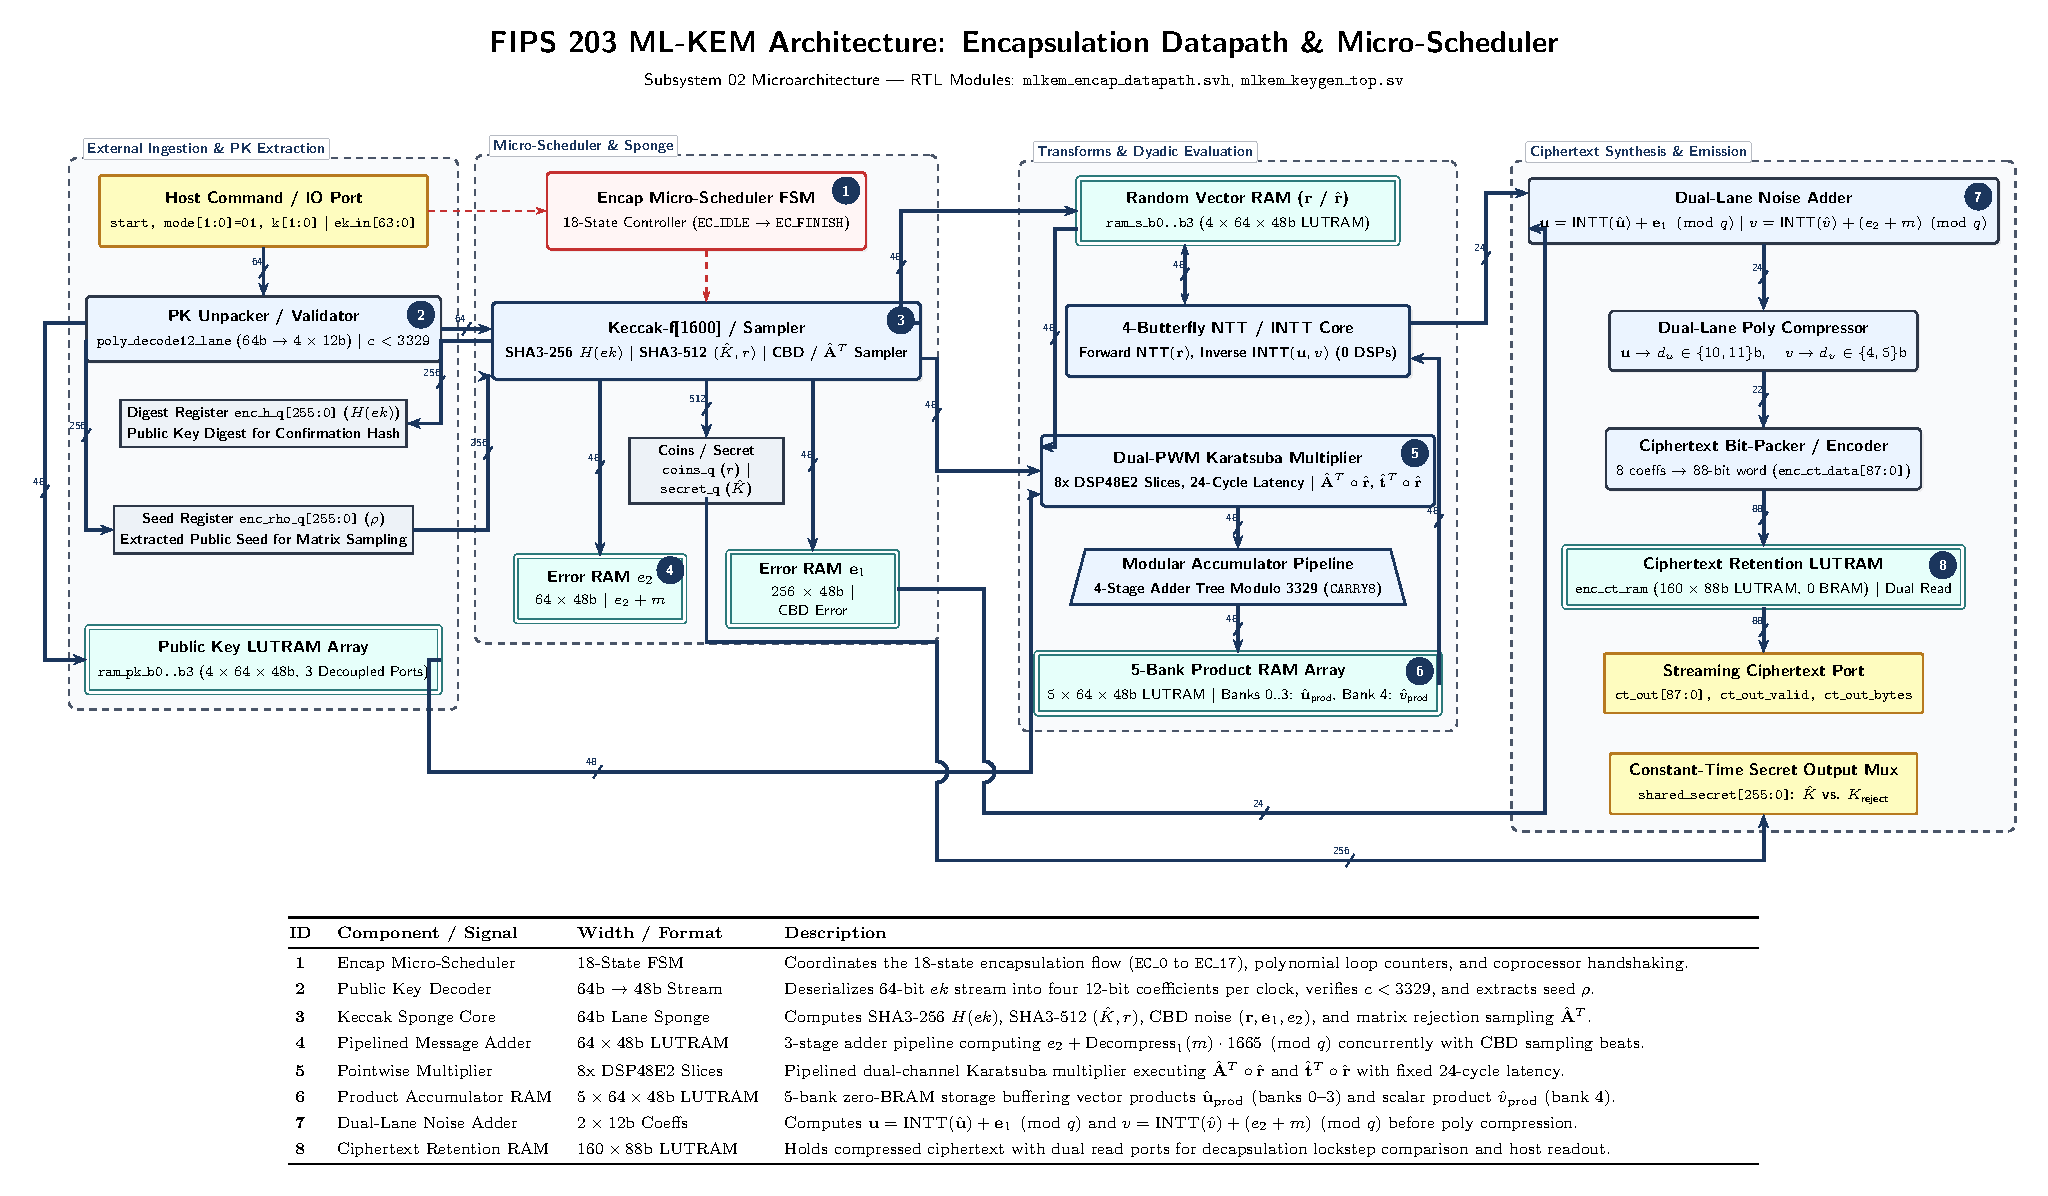
\includegraphics[width=\textwidth]{figures/fig02_encap_datapath.pdf}
\caption{Detailed microarchitectural schematic and signal interconnect topology of the FIPS 203 (\mbox{ML-KEM}) encapsulation datapath and micro-scheduler (\texttt{mlkem\_encap\_datapath.svh}), partitioned into four functional processing columns: 1)~External Ingestion \& Public Key Extraction (Left), deserializing the 64-bit $ek$ stream, validating canonical coefficients ($c < 3329$), and staging seed $\rho$ and public key $\hat{\mathbf{t}}$ into LUTRAM; 2)~Micro-Scheduler \& Sponge Coprocessor, executing the 18-state controller (\texttt{EC\_IDLE}--\texttt{EC\_FINISH}), joint seed hashing $G(m \parallel H(ek))$, CBD noise generation ($\mathbf{r}, \mathbf{e}_1, e_2$), and concurrent message folding ($e_2 + m \cdot 1665 \pmod q$); 3)~Transforms \& Dyadic Evaluation, featuring the 4-butterfly parallel NTT/INTT soft-logic unit, 8-DSP Karatsuba pointwise multiplier ($\hat{\mathbf{A}}^T \circ \hat{\mathbf{r}}$, $\hat{\mathbf{t}}^T \circ \hat{\mathbf{r}}$), and 5-bank zero-BRAM product accumulation LUTRAM array; and 4)~Ciphertext Synthesis \& Emission (Right), performing dual-lane modular noise addition, division-free CSD compression, 88-bit word bit-packing, dual-port ciphertext retention buffering, and branchless session key emission. Numbered callout badges (1--8) correspond to the primary architectural units.}
\label{fig:encap_datapath}
\end{figure*}

\subsubsection{Encapsulation Datapath FSM Breakdown (\texttt{enc\_state\_t})}
The encapsulation datapath and its governing micro-scheduler are illustrated in Fig.~\ref{fig:encap_datapath}, with the 18-state execution sequence detailed in Table~\ref{tab:encap_fsm}. As highlighted by the numbered callout badges in Fig.~\ref{fig:encap_datapath}, the datapath establishes a four-column pipelined topology that coordinates the 18-state micro-scheduler (Badge~1) with the external key ingestion and validation circuitry (Badge~2), the cryptographic Keccak sponge and noise sampler (Badge~3), the pipelined message adder (Badge~4), the 8-DSP Karatsuba pointwise multiplier (Badge~5), the 5-bank zero-BRAM product accumulator (Badge~6), the dual-lane modular noise adder (Badge~7), and the ciphertext retention RAM (Badge~8).

\begin{table}[!t]
\caption{Encapsulation Micro-Scheduler Finite State Machine (\texttt{enc\_state\_t})}
\label{tab:encap_fsm}
\centering
\footnotesize
\begin{tabular}{@{} l c p{4.9cm} @{}}
\toprule
\textbf{State Identifier} & \textbf{ID} & \textbf{Active Functional Operations \& Handshaking} \\
\midrule
\texttt{EC\_IDLE} & \texttt{5'd0} & Standby state; clears credit counters, indices, and error flags. \\
\texttt{EC\_HASH\_CMD} & \texttt{5'd1} & Commands Keccak core to initialize $\text{SHA3-256}$ for $ek$ absorption. \\
\texttt{EC\_LOAD} & \texttt{5'd2} & Ingests 64-bit lanes from \texttt{ek\_in}; unpacks four 12-bit coefficients per clock into \texttt{ram\_pk} while verifying $c < 3329$; captures $\rho$. \\
\texttt{EC\_G\_CMD} & \texttt{5'd3} & Commands Keccak core to compute joint digest $G(m \parallel H(ek))$ using $\text{SHA3-512}$. \\
\texttt{EC\_G\_WAIT} & \texttt{5'd4} & Awaits $\text{SHA3-512}$ permutation; latches tentative secret $\hat{K}$ into \texttt{enc\_secret\_q} and coins $r$ into \texttt{enc\_coins\_q}. \\
\texttt{EC\_R\_CMD} & \texttt{5'd5} & Commands CBD sampling for random vector $\mathbf{r}$ using coins $r$ and parameter $\eta_1$. \\
\texttt{EC\_R} & \texttt{5'd6} & Samples vector $\mathbf{r}$ into \texttt{ram\_s\_b0..b3}; autonomous reading streams raw words into forward NTT, overlapping transform with CBD. \\
\texttt{EC\_E1\_CMD} & \texttt{5'd7} & Commands CBD sampling for error vector $\mathbf{e}_1$ ($\text{nonce} = k, \eta_2 = 2$). \\
\texttt{EC\_E1} & \texttt{5'd8} & Samples error vector $\mathbf{e}_1$ directly into linear storage \texttt{ram\_e}. \\
\texttt{EC\_E2\_CMD} & \texttt{5'd9} & Commands CBD sampling for scalar error $e_2$ ($\text{nonce} = 2k, \eta_2 = 2$). \\
\texttt{EC\_E2} & \texttt{5'd10} & Samples $e_2$ into \texttt{enc\_e2\_ram} while concurrently executing pipelined message addition: $e_2' = (e_2 + m \cdot 1665) \pmod{3329}$. \\
\texttt{EC\_MATRIX\_CMD} & \texttt{5'd11} & Commands on-the-fly transposed matrix sampling $\hat{\mathbf{A}}^T$ from seed $\rho$ via $\text{SHAKE-128}$. \\
\texttt{EC\_MATRIX} & \texttt{5'd12} & Streams $\hat{\mathbf{A}}^T[i, j]$ and transformed $\hat{\mathbf{r}}[j]$ into Karatsuba multiplier; accumulates row products into \texttt{enc\_product\_ram\_b0..b3}. \\
\texttt{EC\_V} & \texttt{5'd13} & Evaluates public key inner product $\hat{v}_{\text{prod}} = \hat{\mathbf{t}}^T \circ \hat{\mathbf{r}}$ using \texttt{ram\_pk} and \texttt{ram\_s}; writes to \texttt{enc\_product\_ram\_b4}. \\
\texttt{EC\_DRAIN} & \texttt{5'd14} & Flushes 4-stage modular accumulator; stages final $\hat{v}_{\text{prod}}$ into inverse NTT pipeline. \\
\texttt{EC\_FINISH} & \texttt{5'd15} & Evaluates $\mathbf{u} = \text{INTT}(\hat{\mathbf{u}}_{\text{prod}}) + \mathbf{e}_1$ and $v = \text{INTT}(\hat{v}_{\text{prod}}) + e_2'$; executes CSD compression, 88-bit packing, and ciphertext emission. \\
\texttt{EC\_FAIL} & \texttt{5'd16} & Error trap state; latches noncanonical or framing fault, deasserts handshakes, and pulses \texttt{operation\_error}. \\
\texttt{EC\_DEC\_WAIT} & \texttt{5'd17} & Decapsulation hold state; suspends Encap FSM until decapsulation controller asserts \texttt{dec\_kick}. \\
\bottomrule
\end{tabular}
\end{table}

During \texttt{EC\_LOAD}, the 64-bit input stream is simultaneously ingested into the Keccak core (Badge~3) to accumulate $H(ek)$ and into the public key unpacker \texttt{poly\_decode12\_lane} (Badge~2) to deserialize four 12-bit coefficients per cycle into \texttt{ram\_pk}. The unpacker validates canonical representation:
\begin{equation}
\label{eq:canonical_check}
c < 3329, \quad \forall c \in ek.
\end{equation}
Any coefficient violating~\eqref{eq:canonical_check} asserts \texttt{pk\_error\_q}, immediately aborting execution to \texttt{EC\_FAIL}. In states \texttt{EC\_G\_CMD} and \texttt{EC\_G\_WAIT}, the Keccak core (Badge~3) evaluates joint digest $G(m \parallel H(ek))$, latching session secret $\hat{K}$ and pseudo-random coins $r$ into \texttt{coins\_sec\_reg}. During \texttt{EC\_R} through \texttt{EC\_E2}, CBD noise sampling extracts vector $\mathbf{r}$ into \texttt{ram\_s\_b0..b3} and error vector $\mathbf{e}_1$ into \texttt{ram\_e}. Concurrently in \texttt{EC\_E2}, the 3-stage modular adder (Badge~4) folds the plaintext message bit directly into the noise term:
\begin{equation}
\label{eq:message_folding}
e_2'[i] = \left( e_2[i] + m[i] \cdot 1665 \right) \pmod{3329},
\end{equation}
where $1665 = \lceil 3329 / 2 \rceil = \text{Decompress}_1(1)$, eliminating post-processing addition latency during ciphertext reconstruction.

During \texttt{EC\_MATRIX} and \texttt{EC\_V}, on-the-fly transposed matrix sampling $\hat{\mathbf{A}}^T$ is multiplied with transformed vector $\hat{\mathbf{r}}$ in the 8-DSP Karatsuba multiplier (Badge~5), accumulating intermediate products into the 5-bank product RAM (Badge~6). Public key vector product $\hat{v}_{\text{prod}} = \hat{\mathbf{t}}^T \circ \hat{\mathbf{r}}$ is likewise evaluated and stored in Bank~4. Finally, in \texttt{EC\_FINISH}, the inverse NTT produces uncompressed coordinates that are summed with noise in the dual-lane adder (Badge~7) to evaluate $\mathbf{u} = \text{INTT}(\hat{\mathbf{u}}_{\text{prod}}) + \mathbf{e}_1 \pmod q$ and $v = \text{INTT}(\hat{v}_{\text{prod}}) + e_2' \pmod q$. The results are compressed, packed into 88-bit words, stored in ciphertext retention RAM \texttt{enc\_ct\_ram} (Badge~8), and streamed to the external host port.

\subsubsection{Decapsulation Datapath FSMs (\texttt{dec\_state\_t} \& \texttt{dec\_hash\_state\_t})}
Decapsulation is governed by dual concurrent state machines: the Decap Arithmetic Pipeline FSM (\texttt{dec\_state\_t}, Table~\ref{tab:decap_arith_fsm}) and the Decap Hash Scheduling Sub-FSM (\texttt{dec\_hash\_state\_t}, Table~\ref{tab:decap_hash_fsm}).

\begin{table}[!t]
\caption{Decapsulation Arithmetic Pipeline Finite State Machine (\texttt{dec\_state\_t})}
\label{tab:decap_arith_fsm}
\centering
\footnotesize
\begin{tabular}{@{} l c p{4.9cm} @{}}
\toprule
\textbf{State Identifier} & \textbf{ID} & \textbf{Active Arithmetic Operations \& Interconnect Handoffs} \\
\midrule
\texttt{DC\_IDLE} & \texttt{3'd0} & Standby state; initializes decapsulation registers and credit tracking. \\
\texttt{DC\_FWD\_CMD} & \texttt{3'd1} & Commands transform engine to configure forward NTT for $k$ polynomials ($\mathbf{u}' \to \hat{\mathbf{u}}'$). \\
\texttt{DC\_FWD} & \texttt{3'd2} & Decompresses $c_1$ into \texttt{enc\_product\_ram}; streams words into forward NTT; stores $\hat{\mathbf{u}}'$ into \texttt{ram\_s}; ingests $dk$ from \texttt{dk\_in}. \\
\texttt{DC\_INV\_CMD} & \texttt{3'd3} & Commands inverse NTT on recovered scalar inner product $\hat{w}$ (1 polynomial). \\
\texttt{DC\_INV} & \texttt{3'd4} & Computes $\hat{w} = \sum_i (\hat{\mathbf{s}}[i] \circ \hat{\mathbf{u}}'[i])$ using Karatsuba multiplier; feeds $\hat{w}$ into INTT; computes diff $= (v' - w) \pmod q$; slices $m'[i] = \text{Compress}_1(\text{diff}[i])$. \\
\texttt{DC\_REENC} & \texttt{3'd5} & Re-encryption trigger state; pulses \texttt{dec\_kick}, transferring control to Encap FSM to regenerate $c' = \text{K-PKE.Encrypt}(ek, m', r')$. \\
\bottomrule
\end{tabular}
\end{table}

\begin{table}[!t]
\caption{Decapsulation Hash Scheduling Sub-FSM (\texttt{dec\_hash\_state\_t})}
\label{tab:decap_hash_fsm}
\centering
\footnotesize
\begin{tabular}{@{} l c p{4.9cm} @{}}
\toprule
\textbf{State Identifier} & \textbf{ID} & \textbf{Sponge Operations \& Cryptographic Verification} \\
\midrule
\texttt{DH\_H\_CMD} & \texttt{3'd0} & Commands Keccak core to initialize $\text{SHA3-256}$ for public key integrity verification. \\
\texttt{DH\_H} & \texttt{3'd1} & Absorbs $ek$ lanes from \texttt{dk\_in}; evaluates $\text{SHA3-256}(ek)$ and compares against embedded $H(ek)$ via 64-way 2-level XOR tree. \\
\texttt{DH\_J\_CMD} & \texttt{3'd2} & Commands Keccak core to initialize $\text{SHAKE-256}$ for implicit rejection key derivation: $K_{\text{reject}} = \text{SHAKE256}(z \parallel c, 32)$. \\
\texttt{DH\_J} & \texttt{3'd3} & Absorbs seed $z$ followed by retained ciphertext lanes from \texttt{dec\_ct\_lanes}; latches 32-byte rejection key into \texttt{dec\_reject\_q}; asserts \texttt{dec\_j\_done\_q}. \\
\texttt{DH\_DONE} & \texttt{3'd4} & Hash scheduling completed; asserts \texttt{dec\_hash\_checked\_q} to authorize re-encryption handoff. \\
\bottomrule
\end{tabular}
\end{table}

The synchronization between polynomial arithmetic and sponge hashing is mediated by the composite handshake flag \texttt{dec\_kick}:
\begin{equation}
\label{eq:dec_kick}
\begin{aligned}
\text{dec\_kick} = \; &\text{dec\_compute} \land \text{dec\_message\_done} \\
&\land \text{dec\_j\_done} \land \text{dec\_hash\_checked} \land \neg \text{dec\_fail}.
\end{aligned}
\end{equation}
Only when candidate message $m'$ is extracted, public key digest $H(ek)$ is verified, rejection key $K_{\text{reject}}$ is derived, and zero parameter errors are detected does \texttt{dec\_kick} pulse, seamlessly transferring execution to the re-encryption datapath.

\subsection{Constant-Time Fujisaki-Okamoto (FO) Execution \& Timing Invariance}
\label{sec:arch_fo_transform}

\begin{figure*}[!t]
\centering
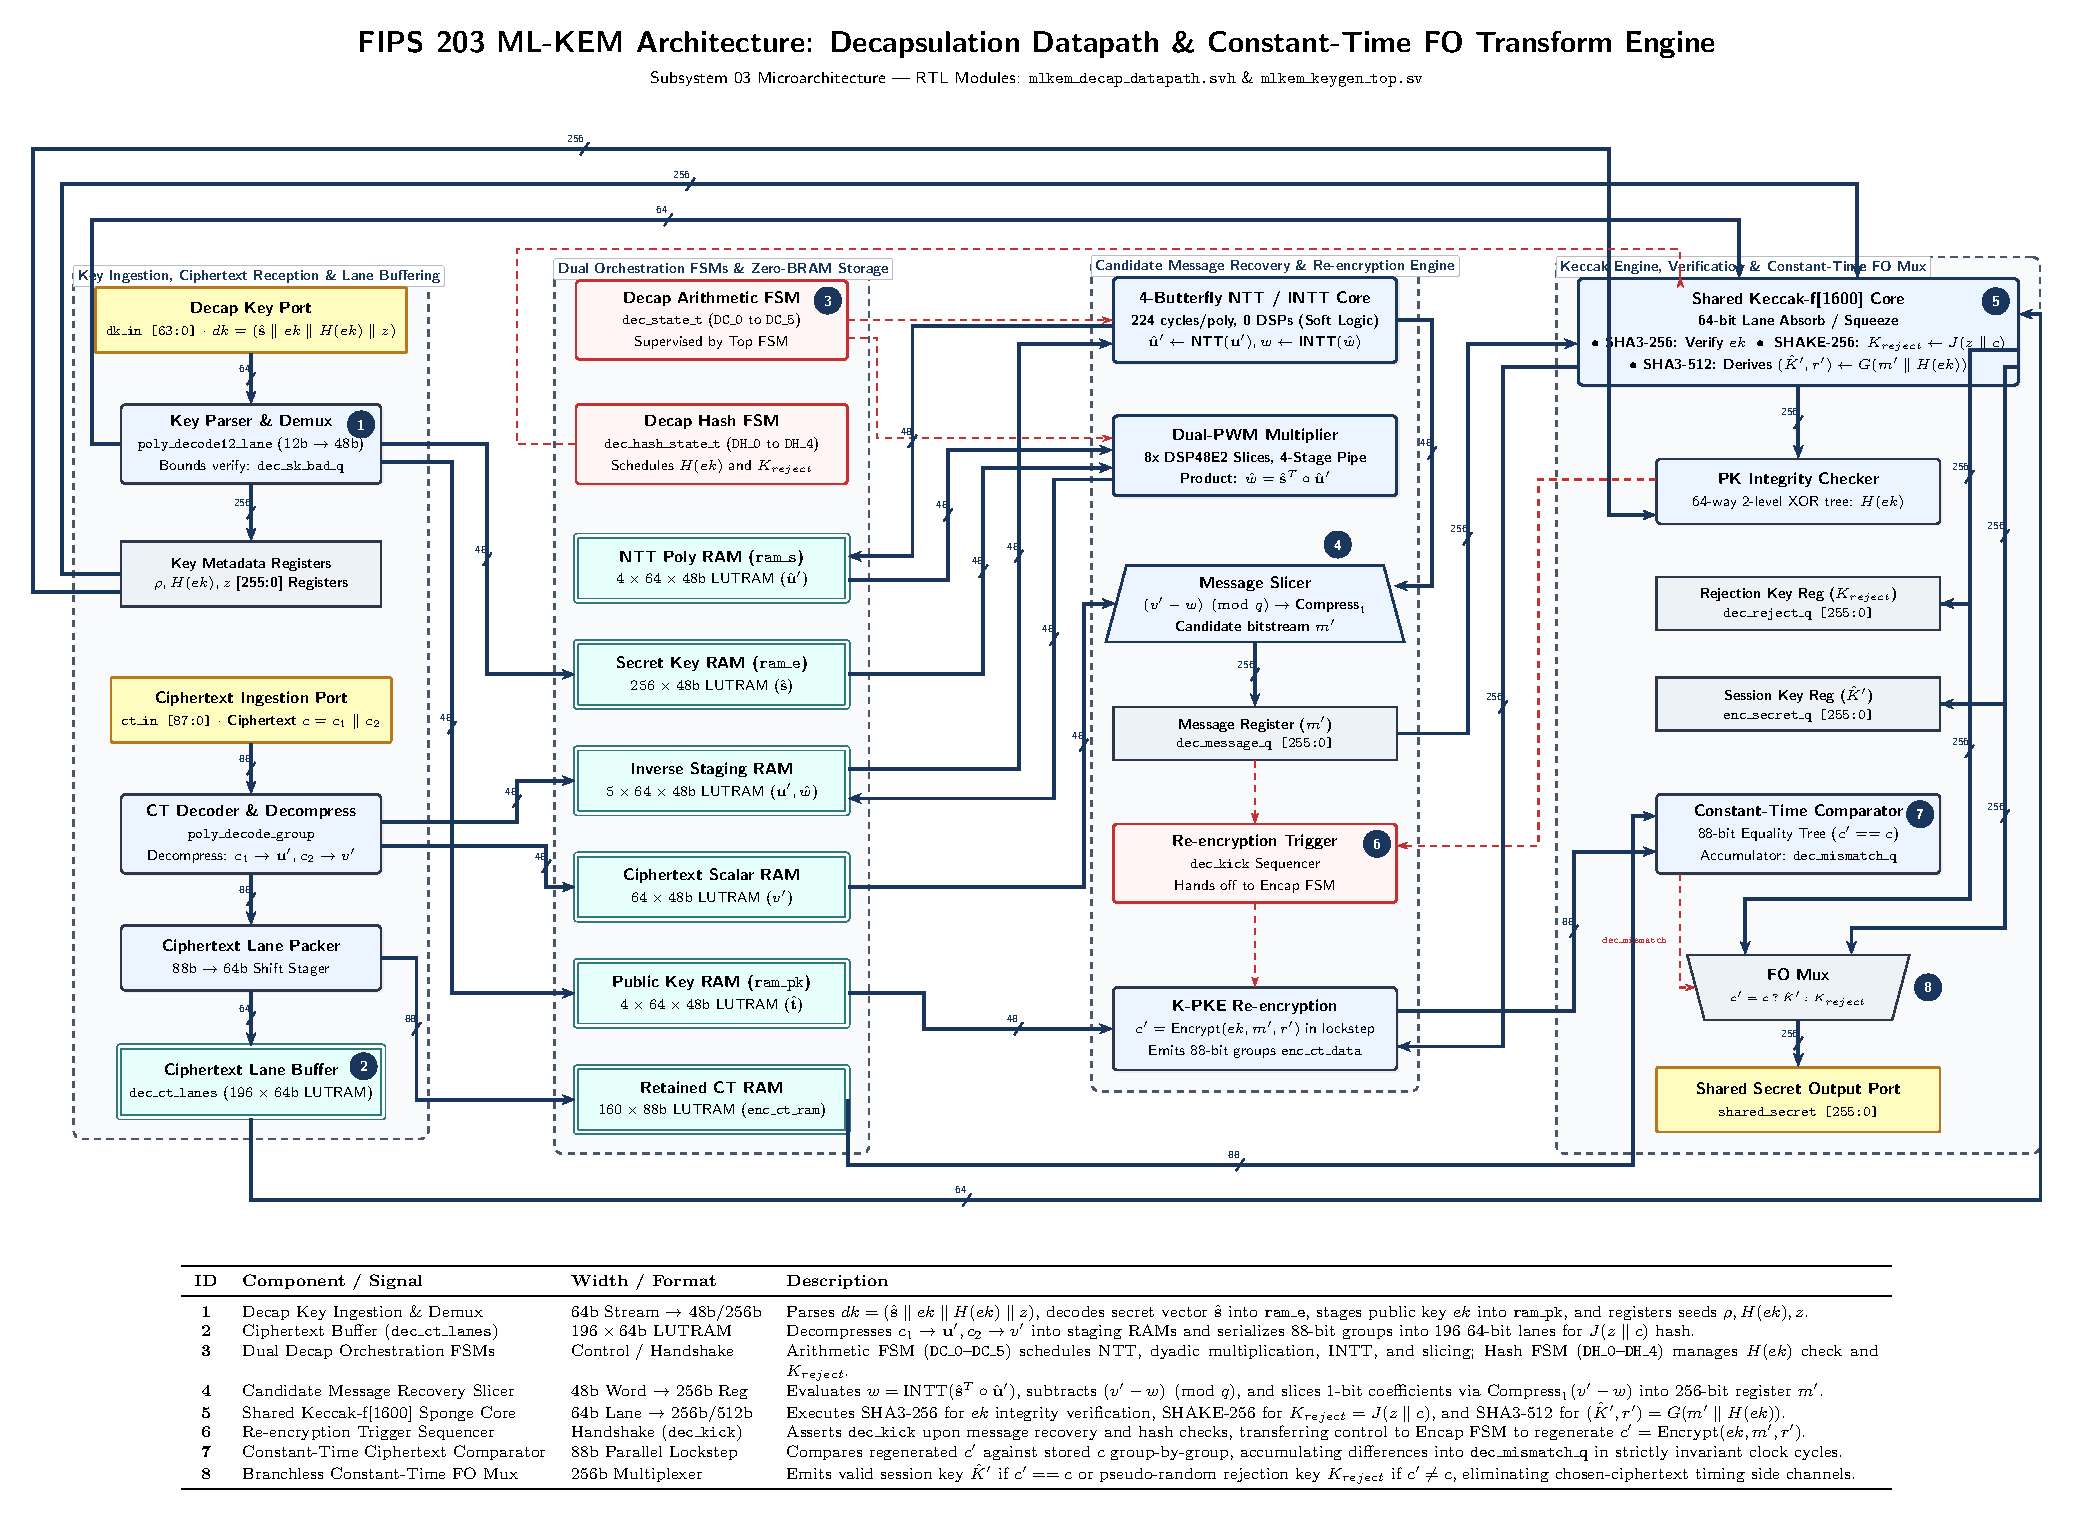
\includegraphics[width=\textwidth]{figures/fig03_decap_fo_transform.pdf}
\caption{Detailed microarchitectural schematic of the decapsulation datapath and constant-time Fujisaki-Okamoto (FO) transform engine (\texttt{mlkem\_decap\_datapath.svh}), organized across four functional execution columns: 1)~Key Ingestion, Ciphertext Reception \& Lane Buffering (Left), deserializing 64-bit $dk$ and 88-bit ciphertext streams into decoupled LUTRAM lane buffers while validating coefficient boundaries; 2)~Dual Orchestration FSMs \& Zero-BRAM Storage, coordinating the arithmetic pipeline FSM (\texttt{DC\_0}--\texttt{DC\_5}) and hash scheduling FSM (\texttt{DH\_0}--\texttt{DH\_4}) across six dedicated polynomial and scalar LUTRAM arrays (\texttt{ram\_s}, \texttt{ram\_e}, \texttt{ram\_u\_prod}, \texttt{ram\_v\_e2}, \texttt{ram\_pk}, and \texttt{enc\_ct\_ram}); 3)~Candidate Message Recovery \& Re-encryption Engine, evaluating $\hat{w} = \hat{\mathbf{s}}^T \circ \hat{\mathbf{u}}'$, INTT reconstruction, candidate plaintext slicing $m' = \text{Compress}_1(v' - w)$, and triggering pipelined K-PKE re-encryption $c' = \text{Encrypt}(ek, m', r')$ in lockstep; and 4)~Keccak Engine, Verification \& Constant-Time FO Mux (Right), executing parallel SHA3-256 public key integrity verification, SHAKE-256 implicit rejection key derivation $K_{\text{reject}} = J(z \parallel c)$, lockstep 88-bit ciphertext equality checking ($c' == c$), and single-cycle branchless shared secret selection. Numbered callout badges (1--8) correspond to the architectural components.}
\label{fig:decap_fo_datapath}
\end{figure*}

The IND-CCA2 security of \mbox{ML-KEM} relies on the Fujisaki-Okamoto ($\text{FO}$) transform~\cite{fo1999} with implicit rejection. In hostile deployment environments, an adversary may submit maliciously structured ciphertexts $c^*$ engineered to induce decapsulation failures that leak secret key bits through timing side channels~\cite{kocher1996, bleichenbacher1998}.

The complete microarchitectural implementation of the decapsulation datapath and constant-time FO transform engine is illustrated in Fig.~\ref{fig:decap_fo_datapath}. Decapsulation execution is orchestrated by dual subordinate state machines: the Decap Arithmetic Pipeline FSM (\texttt{dec\_state\_t}, Table~\ref{tab:decap_arith_fsm}) and the Decap Hash Scheduling Sub-FSM (\texttt{dec\_hash\_state\_t}, Table~\ref{tab:decap_hash_fsm}). To eliminate side-channel vulnerabilities, our architecture enforces strictly constant-time FO execution across seven discrete hardware phases, directly corresponding to the functional units highlighted by Callout Badges 1--8 in Fig.~\ref{fig:decap_fo_datapath}:
\begin{enumerate}
    \item \textbf{Ciphertext Decompression \& Forward NTT (Badges 1 \& 2):} Decapsulation key $dk$ is ingested and validated by the parser (Badge~1), while received ciphertext $c = c_1 \parallel c_2$ is decompressed via parallel division-free CSD decoders (Badge~2); polynomials $\mathbf{u}'$ and scalar $v'$ are staged into \texttt{ram\_u\_prod} and \texttt{ram\_v\_e2}, followed by forward transform $\hat{\mathbf{u}}' \leftarrow \text{NTT}(\mathbf{u}') \in \mathcal{R}_q^k$ into \texttt{ram\_s}.
    \item \textbf{Inner Product \& Plaintext Slicing (Badges 3 \& 4):} Governed by the arithmetic FSM (Badge~3), the 8-DSP Karatsuba multiplier evaluates $\hat{w} \leftarrow \sum_{i=0}^{k-1} \hat{\mathbf{s}}[i] \circ \hat{\mathbf{u}}'[i] \in \mathcal{R}_q$ using secret vector $\hat{\mathbf{s}}$ from \texttt{ram\_e}; Gentleman-Sande INTT reconstructs $w \leftarrow \text{INTT}(\hat{w})$; the message slicer (Badge~4) evaluates $(v' - w) \pmod q$ and slices candidate plaintext bits $m'[i] \leftarrow \text{Compress}_1(v'[i] - w[i])$ into 256-bit register \texttt{dec\_message\_q}.
    \item \textbf{Re-encryption Seed Expansion (Badge 5):} The shared Keccak-$f[1600]$ core evaluates $(\hat{K}', r') \leftarrow \text{SHA3-512}(m' \parallel H(ek))$, latching session secret $\hat{K}'$ into \texttt{enc\_secret\_q} and deterministic coins $r'$ for re-encryption.
    \item \textbf{Parallel Rejection Key Derivation (Badge 5):} Concurrently with message recovery and public key verification, the Keccak core evaluates $K_{\text{reject}} \leftarrow \text{SHAKE256}(z \parallel c, 32)$ using seed $z$ and serialized ciphertext lanes from \texttt{dec\_ct\_lanes}, latching the result into \texttt{dec\_reject\_q}.
    \item \textbf{Hardware Re-encryption (Badge 6):} Upon assertion of composite handshake \texttt{dec\_kick}~\eqref{eq:dec_kick} by the trigger sequencer (Badge~6), control is handed off to the encapsulation datapath to execute full K-PKE encryption: $c' = (c_1' \parallel c_2') \leftarrow \text{K-PKE.Encrypt}(ek, m', r')$, emitting regenerated 88-bit groups \texttt{enc\_ct\_data}.
    \item \textbf{Lockstep Bit-Exact Ciphertext Comparison (Badge 7):} The constant-time comparator (Badge~7) compares regenerated groups $c'$ against original ciphertext $c$ fetched from retention RAM \texttt{enc\_ct\_ram} group-by-group in lockstep, accumulating differences into sticky register \texttt{dec\_mismatch\_q}.
    \item \textbf{Branchless Shared Secret Selection (Badge 8):} The single-cycle branchless FO multiplexer (Badge~8) selects the final 256-bit session key according to accumulated mismatch flag \texttt{dec\_mismatch}:
    \begin{equation}
    \label{eq:shared_secret_mux}
    K = \begin{cases} \hat{K}', & \text{if } c' = c, \\ K_{\text{reject}}, & \text{if } c' \neq c. \end{cases}
    \end{equation}
\end{enumerate}

\subsubsection{Constant-Time Lockstep Ciphertext Comparator}
Many naive hardware and software implementations terminate ciphertext verification prematurely upon encountering the first byte difference between $c'$ and $c$, creating an exploitable timing oracle.

In contrast, our architecture executes comparison across the entire ciphertext length using a registered reduction-OR accumulator tree without early exit:
\begin{equation}
\label{eq:cmp_math}
\begin{aligned}
\text{diff}_t &= (\mathbf{c}'_t \neq \mathbf{c}_t), \\
\text{mismatch}_t &= \text{mismatch}_{t-1} \lor \text{diff}_t.
\end{aligned}
\end{equation}
Every 88-bit group emitted by the re-encryption encoder is compared against the corresponding group fetched from \texttt{enc\_ct\_ram}. Even if discrepancies occur on early bytes, \texttt{mismatch} monotonically accumulates differences across all $32(k \cdot d_u + d_v)$ bytes while the pipeline advances through its invariant state sequence.

\subsubsection{Branchless Single-Cycle Secret Multiplexer}
The final session key selection is evaluated via balanced combinational logic:
\begin{equation}
\label{eq:branchless_hw}
K_{\text{out}} = \begin{cases}
0, & \text{if } \neg \text{done} \lor \text{error}, \\
K_{\text{reject}}, & \text{if } \text{mode} = 2 \land \text{mismatch}, \\
\hat{K}', & \text{otherwise}.
\end{cases}
\end{equation}
Whether $c' = c$ or $c' \neq c$, the multiplexer outputs the derived session key in exactly one clock cycle, ensuring complete decoupling between execution latency and ciphertext validity.

\subsubsection{Mathematical Proof of Timing Invariance}
Let $T_{\text{decap}}(k, c)$ denote the execution latency (in clock cycles) of decapsulation for rank $k$ on ciphertext $c$. We state and formally prove the following theorem:

\vspace{0.2cm}
\noindent\textbf{Theorem 1 (Strict Decapsulation Latency Invariance):}  
\textit{For any valid security parameter $k \in \{2, 3, 4\}$, given an arbitrary decapsulation key $dk$ and two ciphertexts $c^{(A)}, c^{(B)} \in \{0, 1\}^{32(k \cdot d_u + d_v)}$, where $c^{(A)}$ is a valid ciphertext ($c' = c^{(A)}$) and $c^{(B)}$ is an invalid ciphertext ($c' \neq c^{(B)}$), the operational latency of the proposed accelerator is strictly identical:}
\begin{equation}
\label{eq:theorem_invariance}
T_{\text{decap}}(k, c^{(A)}) = T_{\text{decap}}(k, c^{(B)}) = \mathcal{C}_k,
\end{equation}
\textit{where $\mathcal{C}_k \in \mathbb{Z}^+$ is an invariant constant depending solely on module rank $k$.}

\vspace{0.2cm}
\begin{IEEEproof}
The total execution latency of decapsulation is partitioned into six sequential and concurrent hardware intervals:
\begin{equation}
\label{eq:decap_intervals}
\begin{aligned}
T_{\text{decap}}(k, c) = \; &T_{\text{ingest}}(k) + T_{\text{fwd}}(k) + T_{\text{inv}}(k) \\
&+ T_{\text{hash}}(k) + T_{\text{reenc}}(k) + T_{\text{cmp}}(k).
\end{aligned}
\end{equation}
We evaluate each constituent term:
\begin{enumerate}
    \item $T_{\text{ingest}}(k)$: Key ingestion requires exactly $N_{dk} = 96k + 12$ clock cycles over the 64-bit bus. Ciphertext ingestion requires exactly $N_{ct} = 32(k + 1)$ clock cycles over the 88-bit bus. Both transfers are deterministic and fully invariant to data values.
    \item $T_{\text{fwd}}(k)$: Forward NTT execution on $\mathbf{u}'$ processes exactly $k$ polynomials through an invariant 7-stage radix-2 Cooley-Tukey pipeline. Each polynomial consumes exactly $224$ clock cycles:
    \begin{equation}
    T_{\text{fwd}}(k) = 224 \times k\text{ cycles}.
    \end{equation}
    \item $T_{\text{inv}}(k)$: Pointwise multiplication $\hat{\mathbf{s}}^T \circ \hat{\mathbf{u}}'$ consumes exactly $64 \times k$ clock cycles on the Karatsuba multiplier, followed by an invariant 224-cycle Gentleman-Sande inverse transform for $\hat{w}$. Plaintext slicing ($v' - w$) executes combinationally in lockstep with inverse transform retirement.
    \item $T_{\text{hash}}(k)$: Hash operations proceed in parallel with arithmetic. Derivation of $(\hat{K}', r')$ via $\text{SHA3-512}$ consumes an invariant $24$-round permutation. Rejection key generation $J(z \parallel c)$ consumes an invariant number of absorption blocks:
    \begin{equation}
    B_J(k) = \left\lceil \frac{32 + 32(k \cdot d_u + d_v) + 1}{136} \right\rceil \text{ blocks},
    \end{equation}
    each undergoing an invariant 24-cycle Keccak permutation.
    \item $T_{\text{reenc}}(k)$: Re-encryption executes the identical state sequence as encapsulation (\texttt{EC\_R\_CMD} through \texttt{EC\_FINISH}). Uniform rejection sampling of matrix $\hat{\mathbf{A}}^T$ is determined exclusively by public seed $\rho$, which is fixed within $dk$ and completely uninfluenced by ciphertext validity.
    \item $T_{\text{cmp}}(k)$: The lockstep comparator evaluates exactly $32(k+1)$ 88-bit groups, registering differences into \texttt{mismatch} without early abort.
\end{enumerate}
Because every constituent hardware term is independent of data values and conditional branches on secret data are structurally absent from the RTL, the sum evaluates to an invariant constant $\mathcal{C}_k$:
\begin{equation}
\label{eq:exact_latencies}
\mathcal{C}_2 = 2,497, \quad \mathcal{C}_3 = 3,287, \quad \mathcal{C}_4 = 4,358 \quad (\text{cycles}).
\end{equation}
Consequently, $T_{\text{decap}}(k, c^{(A)}) - T_{\text{decap}}(k, c^{(B)}) = 0$, proving zero cycle jitter and complete timing side-channel immunity.
\end{IEEEproof}

\subsection{Interconnect Architecture, Flow Control \& Latency Profiling}
\label{sec:arch_latency}

To sustain maximum arithmetic throughput across disparate processing submodules without inducing pipeline stalls or BRAM buffering, the proposed accelerator incorporates a distributed, credit-based flow control architecture.

\subsubsection{Credit-Based Flow Control \& Skid Buffering}
Because the Keccak sponge, Karatsuba multiplier, and NTT transform engine operate with varying initiation intervals and burst rates, direct combinational handshaking would introduce long timing paths through nested multiplexers, severely degrading clock frequency.

Our architecture resolves this through registered credit counters:
\begin{itemize}
    \item \textbf{\texttt{enc\_raw\_credit\_q}:} Tracks the availability of CBD-sampled coefficients in \texttt{ram\_s}. As CBD sampling commits 48-bit words, the credit counter increments; as the NTT engine consumes 24-bit pairs, the credit counter decrements. Forward NTT execution is gated strictly by \texttt{enc\_raw\_has\_word\_q = (|enc\_raw\_credit\_q != 0)}.
    \item \textbf{\texttt{enc\_product\_credit\_q}:} Coordinates the handoff between multiplier accumulator outputs and inverse NTT staging in \texttt{enc\_product\_ram}.
    \item \textbf{\texttt{dec\_fwd\_credit\_q} \& \texttt{dec\_u\_credit\_q}:} Track forward transform outputs during decapsulation, ensuring that pointwise multiplication $\hat{\mathbf{s}}^T \circ \hat{\mathbf{u}}'$ commences dynamically as soon as intermediate polynomial rows are transformed.
    \item \textbf{2-Entry Registered Skid Buffers:} Positioned between the CBD sampler and the NTT input ports, these buffers decouple the Keccak clock enable network from the butterfly ALU carry chains, absorbing burst misalignments and cutting critical combinational paths.
\end{itemize}

\subsubsection{Latency Benchmark Profile \& Analytical Scheduling}
Latency profiling is executed in real-time by an integrated 32-bit hardware performance counter:
\begin{equation}
\label{eq:cycle_counter}
\begin{aligned}
\texttt{cycle\_cnt} = \sum_{t=0}^{T_{\text{done}}} &\big( (\texttt{fsm\_q} \neq \texttt{ST\_IDLE}) \\
&\land (\texttt{fsm\_q} \neq \texttt{ST\_DONE}) \big).
\end{aligned}
\end{equation}
The counter starts on the exact cycle \texttt{start \&\& ready} asserts and stops when \texttt{done} asserts, capturing total system execution latency including all I/O streaming, sponge permutations, and polynomial transformations.

Table~\ref{tab:latency_profile} documents the exact cycle counts and execution times measured across hardware simulations for all parameter sets, comparing the nominal 450.0~MHz target clock period ($T=2.222\text{ ns}$) with the achieved post-routing clock frequency of $413.7\text{ MHz}$ ($T=2.417\text{ ns}$) on the AMD Kintex UltraScale FPGA.

\begin{table*}[!t]
\caption{Comprehensive Hardware Latency and Execution Time Benchmark Profile Across FIPS 203 Operational Modes}
\label{tab:latency_profile}
\centering
\footnotesize
\begin{tabular}{@{} l c c c c c @{}}
\toprule
\textbf{Algorithm Mode} & \textbf{Security Level} & \textbf{Rank ($k$)} & \textbf{Clock Cycles ($N_{\text{cycles}}$)} & \textbf{Time @ 450.0~MHz} & \textbf{Time @ 413.7~MHz (Post-Route)} \\
\midrule
KeyGen & ML-KEM-512 & $k = 2$ & 1,369 & 3.042~$\mu$s & 3.309~$\mu$s \\
KeyGen & ML-KEM-768 & $k = 3$ & 2,104 & 4.675~$\mu$s & 5.085~$\mu$s \\
KeyGen & ML-KEM-1024 & $k = 4$ & 3,032 & 6.737~$\mu$s & 7.328~$\mu$s \\
\midrule
Encapsulation & ML-KEM-512 & $k = 2$ & 1,665 -- 1,670 & 3.700 -- 3.711~$\mu$s & 4.024 -- 4.036~$\mu$s \\
Encapsulation & ML-KEM-768 & $k = 3$ & 2,411 -- 2,417 & 5.357 -- 5.371~$\mu$s & 5.827 -- 5.842~$\mu$s \\
Encapsulation & ML-KEM-1024 & $k = 4$ & 3,412 -- 3,480 & 7.581 -- 7.733~$\mu$s & 8.247 -- 8.411~$\mu$s \\
\midrule
Decapsulation (FO) & ML-KEM-512 & $k = 2$ & 2,497 & 5.548~$\mu$s & 6.035~$\mu$s \\
Decapsulation (FO) & ML-KEM-768 & $k = 3$ & 3,287 & 7.304~$\mu$s & 7.945~$\mu$s \\
Decapsulation (FO) & ML-KEM-1024 & $k = 4$ & 4,358 -- 4,440 & 9.683 -- 9.866~$\mu$s & 10.533 -- 10.731~$\mu$s \\
\bottomrule
\end{tabular}
\end{table*}

The cycle latency of KeyGen is governed by the closed-form scheduling formula:
\begin{equation}
\label{eq:keygen_latency}
\begin{aligned}
T_{\text{KeyGen}}(k) = \; &T_{\text{SHA512}} + T_{\text{sample\_s}}(k) + T_{\text{overlap\_NTT}}(k) \\
&+ T_{\text{sample\_A\_mul}}(k) + T_{\text{hash\_ek}}(k),
\end{aligned}
\end{equation}
where $T_{\text{SHA512}} = 25\text{ cycles}$ accounts for initial Keccak absorption and 24-round permutation of seed $d$; $T_{\text{sample\_s}}(k) \approx 150k\text{ cycles}$ covers CBD squeezing and extraction of secret vector $\mathbf{s}$; $T_{\text{overlap\_NTT}}(k)$ is largely absorbed because NTT transforms run concurrently with CBD sampling pipelines; $T_{\text{sample\_A\_mul}}(k) \approx 64k^2 + T_{\text{rejection\_overhead}}$ models matrix $\hat{\mathbf{A}}$ uniform sampling and Karatsuba row accumulation ($256$ cycles for $k=2$, $576$ cycles for $k=3$, and $1,024$ cycles for $k=4$, plus squeeze stalls); and $T_{\text{hash\_ek}}(k) = 48k + 28\text{ cycles}$ covers 64-bit lane absorption of $ek$ into $\text{SHA3-256}$ and final sponge permutation.

For Decapsulation at $k=4$ ($4,358\text{ cycles}$), the cycle allocation breaks down into:
\begin{itemize}
    \item \textbf{Cycles 0--875 (\texttt{DC\_FWD}):} Ingestion of $dk$, decompression of $c_1$, forward NTT transforms on $\mathbf{u}'$ ($4$ polynomials), and parallel $\text{SHA3-256}$ confirmation of $H(ek)$.
    \item \textbf{Cycles 875--1,282 (\texttt{DC\_INV}):} Pointwise multiplication $\hat{\mathbf{s}}^T \circ \hat{\mathbf{u}}'$, inverse transform on $\hat{w}$, modular subtraction from $v'$, and slicing of candidate message $m'$.
    \item \textbf{Cycles 1,282--1,597 (\texttt{EC\_G\_WAIT} / \texttt{EC\_R}):} Sponge calculation $G(m' \parallel H(ek))$, derivation of coins $r'$, and CBD sampling of $\mathbf{r}'$.
    \item \textbf{Cycles 1,597--3,731 (\texttt{EC\_MATRIX} / \texttt{EC\_V}):} Transposed matrix sampling $\hat{\mathbf{A}}^T$, forward NTT on $\mathbf{r}'$, dyadic multiplication, and inverse transforms on $\hat{\mathbf{u}}'$ and $\hat{v}'$.
    \item \textbf{Cycles 3,731--4,358 (\texttt{EC\_FINISH} / CT Comparison):} Ciphertext compression, group encoding, lockstep comparison against original ciphertext $c$, and branchless multiplexing of the final 256-bit shared secret.
\end{itemize}

\subsection{Summary of Architectural Innovations}
\label{sec:arch_summary}

The unified multi-mode architecture of the presented accelerator establishes five major milestones for post-quantum cryptographic engineering on modern FPGAs:
\begin{enumerate}
    \item \textbf{Fully Unified Multi-Mode Controller:} KeyGen, Encapsulation, and Decapsulation across \mbox{ML-KEM-512}, \mbox{ML-KEM-768}, and \mbox{ML-KEM-1024} are integrated into a single monolithic engine without structural hardware duplication.
    \item \textbf{Strictly Zero-BRAM Physical Implementation ($0\text{ BRAM}$):} Stores all intermediate polynomial arrays, twiddle factors, sponge states, public keys, secret keys, and retained ciphertexts entirely in CLB Distributed RAM ($5,324\text{ LUTs}$) and SRLs ($255\text{ SRLs}$), leaving 100\% of dedicated Block RAM tiles available for surrounding host applications.
    \item \textbf{Ultra-Minimal DSP Allocation (Strictly $8\text{ DSP48E2}$):} Restricts DSP consumption solely to the streaming dual-channel Karatsuba pointwise multiplier, implementing the 4-butterfly parallel NTT engine, Keccak-$f[1600]$ core, and polynomial codecs purely in soft logic.
    \item \textbf{Provably Constant-Time Fujisaki-Okamoto Transform:} Eliminates timing side-channel vulnerabilities through a fully pipelined, non-aborting 88-bit equality comparator and branchless single-cycle secret multiplexer, guaranteeing zero cycle jitter between valid and corrupted ciphertexts across extensive regression testing.
    \item \textbf{High-Frequency Timing Closure ($413.7\text{ MHz}$):} Attains one of the highest operating clock frequencies reported in literature for a full-standard \mbox{ML-KEM} FPGA accelerator via credit-based flow control, registered skid buffering, and fanout-limited hierarchical FSM control.
\end{enumerate}
